% A shift of theta by a constant leaves every gap and G_f unchanged; a shift of theta_1 alone does not.
% Source of the figure, typeset in the paper's own fonts (T1, Latin Modern, 11pt) at the paper's text
% width (6.5in), so \includegraphics does not rescale it. Illustrates CLH-2; it adds no assertion.
% Every coordinate and printed number is read from values that Lean evaluated (Conj43.crossEdges, the gaps and the gradient);
% inputs: f-bar=(3,5,1,2,4), theta/pi=(0,0.1,0.7,0.3,0.8).
% SHA-256 (first 16 hex digits) of the output lines the values come from: gauge_const 00489d65bf4912a5, gauge_e1 8ac3ae195ed7f138.
% Real-valued quantities are floating-point values computed in Lean from the paper's formulas.
% Build: pdflatex <this file> && pdftocairo -svg <this file>.pdf <this file>.svg
\documentclass[11pt]{standalone}
\usepackage[T1]{fontenc}
\usepackage{lmodern}
\usepackage{amsmath,amssymb}
\usepackage{tikz}
\usetikzlibrary{arrows.meta,positioning,calc}

% the palette of the paper's other figures: blue solid for the first curve or strand, ochre dashed for the second
\definecolor{ink}{HTML}{233740}
\definecolor{muted}{HTML}{65757D}
\definecolor{pblue}{HTML}{0072B2}
\definecolor{qochre}{HTML}{B87827}

\tikzset{
  frm/.style={draw=muted, line width=0.5pt},
  axl/.style={draw=muted!70, line width=0.4pt},
  crvP/.style={draw=pblue, line width=1.1pt, line join=round},
  crvQ/.style={draw=qochre, line width=1.1pt, dash pattern=on 4pt off 1.6pt},
  drop/.style={draw=muted, line width=0.4pt, dash pattern=on 1pt off 1.4pt},
  dotQ/.style={circle, fill=qochre, draw=qochre, inner sep=0pt, minimum size=4.2pt},
  dotP/.style={circle, fill=pblue, draw=pblue, inner sep=0pt, minimum size=4.2pt},
  openQ/.style={circle, fill=white, draw=qochre, line width=0.8pt, inner sep=0pt, minimum size=4.2pt},
  lab/.style={font=\footnotesize, inner sep=1.5pt, text=ink},
  labm/.style={font=\small, inner sep=1.5pt, text=ink},
  labQ/.style={font=\footnotesize, inner sep=1.5pt, text=qochre},
  labP/.style={font=\footnotesize, inner sep=1.5pt, text=pblue},
  tick/.style={font=\footnotesize, inner sep=1.2pt, text=muted},
  vtx/.style={circle, draw=ink, fill=white, line width=0.6pt, inner sep=0pt, minimum size=15pt, font=\small, text=ink},
  arrP/.style={pblue, line width=1.0pt, -{Stealth[length=5pt,width=4.2pt]}},
}

\begin{document}
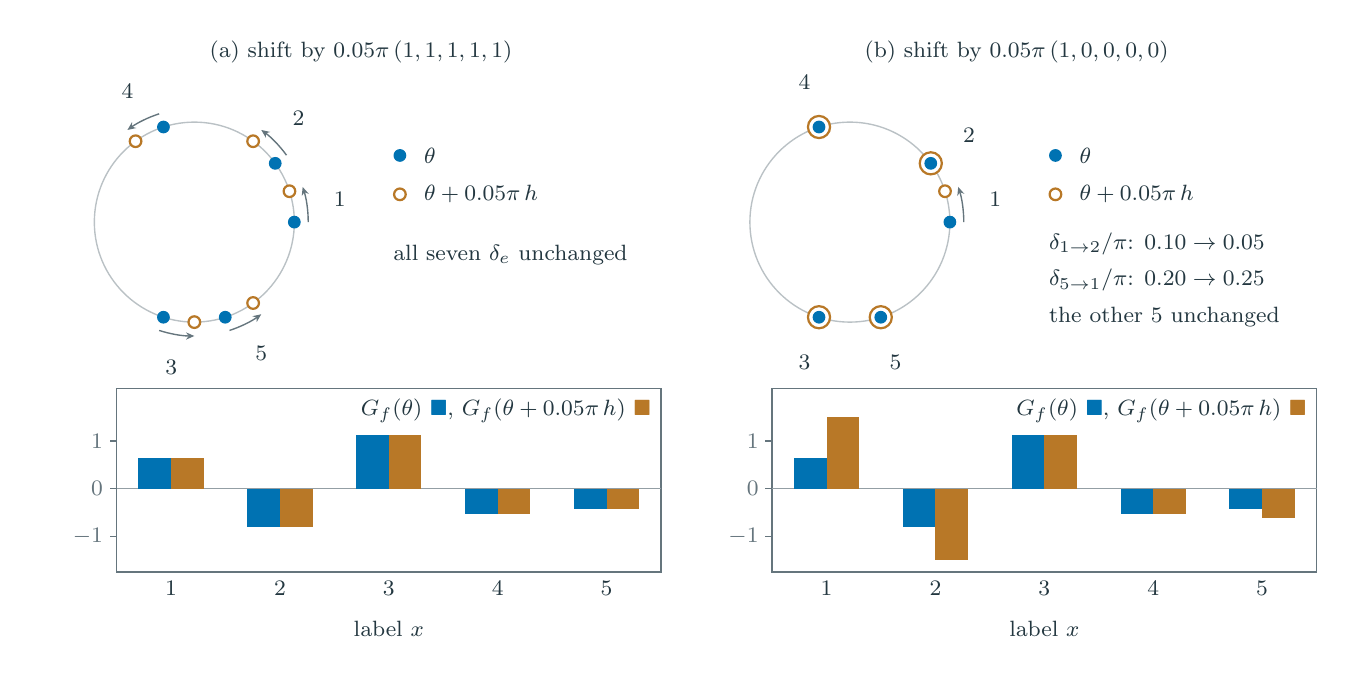
\begin{tikzpicture}[x=1bp,y=1bp]
\useasboundingbox (0,0) rectangle (468.005,222.0025);
\node[lab, anchor=north] at (120.00,219.00) {(a) shift by $0.05\pi\,(1,1,1,1,1)$};
% circ Ca 60.00 152.00 36.00
\draw[draw=muted!45, line width=0.5pt] (60.00,152.00) circle (36.00);
\draw[draw=muted, line width=0.5pt, -{Stealth[length=3pt,width=2.6pt]}] (101.00,152.00) arc[start angle=0.00, end angle=18.00, radius=41.00];
\node[openQ] at (94.24,163.12) {}; %pol Ca after 0 60.00 152.00 36.00
\node[dotP] at (96.00,152.00) {}; %pol Ca before 0 60.00 152.00 36.00
\draw[draw=muted, line width=0.5pt, -{Stealth[length=3pt,width=2.6pt]}] (93.17,176.10) arc[start angle=36.00, end angle=54.00, radius=41.00];
\node[openQ] at (81.16,181.12) {}; %pol Ca after 1 60.00 152.00 36.00
\node[dotP] at (89.12,173.16) {}; %pol Ca before 1 60.00 152.00 36.00
\draw[draw=muted, line width=0.5pt, -{Stealth[length=3pt,width=2.6pt]}] (47.33,113.01) arc[start angle=252.00, end angle=270.00, radius=41.00];
\node[openQ] at (60.00,116.00) {}; %pol Ca after 2 60.00 152.00 36.00
\node[dotP] at (48.88,117.76) {}; %pol Ca before 2 60.00 152.00 36.00
\draw[draw=muted, line width=0.5pt, -{Stealth[length=3pt,width=2.6pt]}] (47.33,190.99) arc[start angle=108.00, end angle=126.00, radius=41.00];
\node[openQ] at (38.84,181.12) {}; %pol Ca after 3 60.00 152.00 36.00
\node[dotP] at (48.88,186.24) {}; %pol Ca before 3 60.00 152.00 36.00
\draw[draw=muted, line width=0.5pt, -{Stealth[length=3pt,width=2.6pt]}] (72.67,113.01) arc[start angle=288.00, end angle=306.00, radius=41.00];
\node[openQ] at (81.16,122.88) {}; %pol Ca after 4 60.00 152.00 36.00
\node[dotP] at (71.12,117.76) {}; %pol Ca before 4 60.00 152.00 36.00
\node[lab, anchor=center] at (112.35,160.29) {$1$};
\node[lab, anchor=center] at (97.48,189.48) {$2$};
\node[lab, anchor=center] at (51.71,99.65) {$3$};
\node[lab, anchor=center] at (35.94,199.22) {$4$};
\node[lab, anchor=center] at (84.06,104.78) {$5$};
\node[dotP] at (134.00,176.00) {};
\node[lab, anchor=west] at (141.00,176.00) {$\theta$};
\node[openQ] at (134.00,162.00) {};
\node[lab, anchor=west] at (141.00,162.00) {$\theta+0.05\pi\,h$};
\node[lab, anchor=west] at (130.00,140.00) {all seven $\delta_e$ unchanged}; %val gaps_unchanged 0 7
% map Ga 32.0000 56.0000 39.2000 17.1429
\draw[frm] (32.00,26.00) rectangle (228.00,92.00);
\draw[axl] (32.00,56.00) -- (228.00,56.00);
\draw[frm] (32.00,38.86) -- (29.50,38.86);
\node[tick, anchor=east] at (28.50,38.86) {$-1$};
\draw[frm] (32.00,56.00) -- (29.50,56.00);
\node[tick, anchor=east] at (28.50,56.00) {$0$};
\draw[frm] (32.00,73.14) -- (29.50,73.14);
\node[tick, anchor=east] at (28.50,73.14) {$1$};
\node[lab, anchor=north] at (51.60,24.50) {$1$};
\node[lab, anchor=north] at (90.80,24.50) {$2$};
\node[lab, anchor=north] at (130.00,24.50) {$3$};
\node[lab, anchor=north] at (169.20,24.50) {$4$};
\node[lab, anchor=north] at (208.40,24.50) {$5$};
\node[lab, anchor=north] at (130.00,10.00) {label $x$};
\fill[fill=pblue] (39.84,56.00) rectangle (51.60,67.02); %bar Ga before 0
\fill[fill=qochre] (51.60,56.00) rectangle (63.36,67.02); %bar Ga after 0
\fill[fill=pblue] (79.04,56.00) rectangle (90.80,42.20); %bar Ga before 1
\fill[fill=qochre] (90.80,56.00) rectangle (102.56,42.20); %bar Ga after 1
\fill[fill=pblue] (118.24,56.00) rectangle (130.00,75.27); %bar Ga before 2
\fill[fill=qochre] (130.00,56.00) rectangle (141.76,75.27); %bar Ga after 2
\fill[fill=pblue] (157.44,56.00) rectangle (169.20,46.89); %bar Ga before 3
\fill[fill=qochre] (169.20,56.00) rectangle (180.96,46.89); %bar Ga after 3
\fill[fill=pblue] (196.64,56.00) rectangle (208.40,48.61); %bar Ga before 4
\fill[fill=qochre] (208.40,56.00) rectangle (220.16,48.61); %bar Ga after 4
\node[lab, anchor=north east] at (226.00,90.00) {$G_f(\theta)$ \textcolor{pblue}{$\blacksquare$}, $G_f(\theta+0.05\pi\,h)$ \textcolor{qochre}{$\blacksquare$}};
\node[lab, anchor=north] at (356.00,219.00) {(b) shift by $0.05\pi\,(1,0,0,0,0)$};
% circ Cb 296.00 152.00 36.00
\draw[draw=muted!45, line width=0.5pt] (296.00,152.00) circle (36.00);
\draw[draw=muted, line width=0.5pt, -{Stealth[length=3pt,width=2.6pt]}] (337.00,152.00) arc[start angle=0.00, end angle=18.00, radius=41.00];
\node[openQ] at (330.24,163.12) {}; %pol Cb after 0 296.00 152.00 36.00
\node[dotP] at (332.00,152.00) {}; %pol Cb before 0 296.00 152.00 36.00
\node[openQ, minimum size=8pt] at (325.12,173.16) {}; %pol Cb after 1 296.00 152.00 36.00
\node[dotP] at (325.12,173.16) {}; %pol Cb before 1 296.00 152.00 36.00
\node[openQ, minimum size=8pt] at (284.88,117.76) {}; %pol Cb after 2 296.00 152.00 36.00
\node[dotP] at (284.88,117.76) {}; %pol Cb before 2 296.00 152.00 36.00
\node[openQ, minimum size=8pt] at (284.88,186.24) {}; %pol Cb after 3 296.00 152.00 36.00
\node[dotP] at (284.88,186.24) {}; %pol Cb before 3 296.00 152.00 36.00
\node[openQ, minimum size=8pt] at (307.12,117.76) {}; %pol Cb after 4 296.00 152.00 36.00
\node[dotP] at (307.12,117.76) {}; %pol Cb before 4 296.00 152.00 36.00
\node[lab, anchor=center] at (348.35,160.29) {$1$};
\node[lab, anchor=center] at (338.88,183.15) {$2$};
\node[lab, anchor=center] at (279.62,101.59) {$3$};
\node[lab, anchor=center] at (279.62,202.41) {$4$};
\node[lab, anchor=center] at (312.38,101.59) {$5$};
\node[dotP] at (370.00,176.00) {};
\node[lab, anchor=west] at (377.00,176.00) {$\theta$};
\node[openQ] at (370.00,162.00) {};
\node[lab, anchor=west] at (377.00,162.00) {$\theta+0.05\pi\,h$};
\node[lab, anchor=west] at (366.00,144.00) {$\delta_{1{\to}2}/\pi$: $0.10\to0.05$}; %val gap 0 0.10 0.05
\node[lab, anchor=west] at (366.00,131.00) {$\delta_{5{\to}1}/\pi$: $0.20\to0.25$}; %val gap 5 0.20 0.25
\node[lab, anchor=west] at (366.00,118.00) {the other 5 unchanged};
% map Gb 268.0000 56.0000 39.2000 17.1429
\draw[frm] (268.00,26.00) rectangle (464.00,92.00);
\draw[axl] (268.00,56.00) -- (464.00,56.00);
\draw[frm] (268.00,38.86) -- (265.50,38.86);
\node[tick, anchor=east] at (264.50,38.86) {$-1$};
\draw[frm] (268.00,56.00) -- (265.50,56.00);
\node[tick, anchor=east] at (264.50,56.00) {$0$};
\draw[frm] (268.00,73.14) -- (265.50,73.14);
\node[tick, anchor=east] at (264.50,73.14) {$1$};
\node[lab, anchor=north] at (287.60,24.50) {$1$};
\node[lab, anchor=north] at (326.80,24.50) {$2$};
\node[lab, anchor=north] at (366.00,24.50) {$3$};
\node[lab, anchor=north] at (405.20,24.50) {$4$};
\node[lab, anchor=north] at (444.40,24.50) {$5$};
\node[lab, anchor=north] at (366.00,10.00) {label $x$};
\fill[fill=pblue] (275.84,56.00) rectangle (287.60,67.02); %bar Gb before 0
\fill[fill=qochre] (287.60,56.00) rectangle (299.36,81.86); %bar Gb after 0
\fill[fill=pblue] (315.04,56.00) rectangle (326.80,42.20); %bar Gb before 1
\fill[fill=qochre] (326.80,56.00) rectangle (338.56,30.53); %bar Gb after 1
\fill[fill=pblue] (354.24,56.00) rectangle (366.00,75.27); %bar Gb before 2
\fill[fill=qochre] (366.00,56.00) rectangle (377.76,75.27); %bar Gb after 2
\fill[fill=pblue] (393.44,56.00) rectangle (405.20,46.89); %bar Gb before 3
\fill[fill=qochre] (405.20,56.00) rectangle (416.96,46.89); %bar Gb after 3
\fill[fill=pblue] (432.64,56.00) rectangle (444.40,48.61); %bar Gb before 4
\fill[fill=qochre] (444.40,56.00) rectangle (456.16,45.44); %bar Gb after 4
\node[lab, anchor=north east] at (462.00,90.00) {$G_f(\theta)$ \textcolor{pblue}{$\blacksquare$}, $G_f(\theta+0.05\pi\,h)$ \textcolor{qochre}{$\blacksquare$}};
\end{tikzpicture}
\end{document}
